\documentclass{article}

\usepackage{mat437pres}


\title{Complex Dynamics}
\author{Lexi Reed and Brian Zhang}
\date{May 2021}

\begin{document}


\maketitle

\section{Julia and Mandelbrot Set Definitions}

Let $P_c(z) = z^2 + c$

Julia set for $P_c$, fixes $c$
\[ J_c = \{ z \mid  \abs{ P_c^n(z) }_n \textrm{bounded} \} \] 


Mandelbrot set instead fixes $z$
\[ M = \{ c \mid \abs{ P_c^n(0) }_n \textrm{bounded} \} \]

To be more precise
\begin{itemize}
    \item Def above is the "filled-in" Julia set
    \item "True" Julia set is the boundary
    \item Above is a Quadratic Julia set, can use other rational functions (ratio of complex polynomials)
\end{itemize}


\section{Julia Set Fractal Nature}

Sequence $z_n = P_c^n(z_0)$, iterating $P_c$ for a given $z_0$ in the Julia set.

Easier to visualize the pre-image (single iteration) of a point $z_n = P_c^{-1}(z_{n + 1})$
\begin{align*}
    z_{n + 1} &= \left( \abs{z_n}e^{i\Arg{z}}\right)^2 + c \\
    z_{n + 1} - c &= \abs{z_n}^2e^{i2\Arg{z}}
\end{align*}
Solving for $z_n$ in terms of $z_{n+1} - c$
\begin{align*}
    2\Arg{z_n} &= \Arg(z_{n+1} - c) + 2\pi k \\
    \Arg{z_n} &= .5 \Arg(z_{n+1} - c) + \pi k,\ k \in \{0, 1\} \\
    \abs{z_n} &= \sqrt{\abs{z_{n+1} - c}}
\end{align*}

We can iterate taking the pre-image of a set containing $J_c$ to approach its shape,
\begin{itemize}
    \item Take nbhd of infinity $S$ s.t. $J_c \subset \complexes - S$
    \item $z_0 \not \in J_c \iff \exists N \ni \forall n > N,\ z_n \in S$
    \item $\complexes - J_c = \bigcup_n P_c^{-n}(S)$
    \item DeMorgan's, pre-image of complement: $J_c = \bigcap_n P_c^{-n}(\complexes - S)$
    % \item Can be visualized as moving towards brighter orange bands in Fig \ref{fig:julia_escape}
\end{itemize}


\begin{figure}[h!]
    \centering
    
\includegraphics[width=.4\linewidth]{images/600px-Time_escape_Julia_set.jpg}
    \caption{Julia set, bands around set indicate "escape" iterations \cite{JuliaTimeEscape}}
    \label{fig:julia_escape}
\end{figure}

Karl Sims gives a visualization for a disk in Fig \ref{fig:karlsims_preimage}. For one iteration,
\begin{itemize}
    \item Translate the disk by $-c$, halve angle for each point, shift radius towards $1$ for each point
    \item Mirror across real axis (pre-image maps one point to two with $\pi$ arg offset)
\end{itemize}

\begin{figure}[htbp!]
    \setlength{\abovecaptionskip}{0pt}
    \captionsetup[subfigure]{labelformat=empty}
    \centering
    \subfloat[]{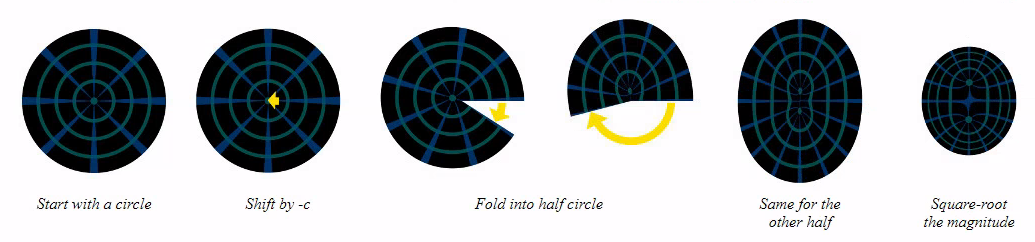
\includegraphics[width=.8\linewidth]{images/karlsimsfold1.png}} \\[-3ex]%
    \subfloat[]{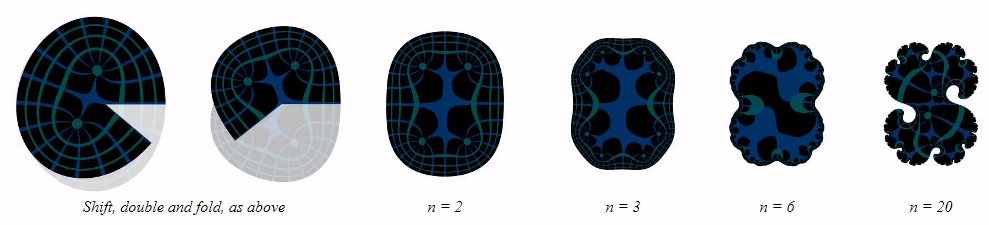
\includegraphics[width=.8\linewidth]{images/karlsimsfold2.png}}%
    \caption{Approaching Julia set by pre-images of disk \cite{KarlSims}} %
    \label{fig:karlsims_preimage}%
\end{figure}%



\section{Julia Set Escape Radius}

How big does the disk need to be such that $J_c \subset D[0, R]$?
\begin{itemize}
    \item Called "Escape Radius"
    \item Find $R$ where $z_0 \not \in D[0, R] \implies \abs{z_{n+1}} > \abs{z_n}$
\end{itemize}

For $P_c(z) = z^2 + 1$, take $\abs{z_n} > \abs{R} > 1$,
\begin{align*}
    \abs{z_{n+1}} &\geq \abs{z_n^2} - \abs{c} &&\text{Reverse Triangle Inequality} \\
    &\geq \abs{z_n^2} - \abs{z_n}\frac{\abs{z_n}}{R}\abs{c} \\
    &= \abs{z_n}\frac{\abs{z_n}}{R}(R - \abs{c})
\end{align*}
Thus $R > 1 + \abs{c} \implies \abs{z_{n+1}} > \abs{z_n}$ \cite{JuliaEscapeRadiusProof}. 

Plotting algorithm: take points in disk, iterate $P_c$, remove points that "escape" the disk.


\section{Julia Set Connectedness}
\begin{itemize}
    \item Julia Set is either connected (Fatou Set)...
    \begin{itemize}
      \item Start from $D[0, R]$, each pre-image iteration preserves connectedness
    \end{itemize}
  
    \item Or something that's like the Cantor set (Fatou Dust)
    \begin{itemize}
      \item Start from $D[0, R]$, each pre-image iteration cuts the previous pieces in two
    \end{itemize}

    \item If $0 \in J_c$, then it's connected, otherwise Fatou Dust
    \item $J_c\ \textrm{connected} \iff 0 \in J_c \iff c \in M$ (M is Mandelbrot set)
\end{itemize}

\begin{figure}[!h]
    
\includegraphics[width=\linewidth]{images/Cantor_set_in_seven_iterations.png}
    \caption{Cantor set interval visualization \cite{Cantor}}%\label{fig:boat1}
\end{figure}

\begin{figure}[!htbp]
    \centering
    
\includegraphics[width=.4\linewidth]{images/julia_fatou_dust_c_45_1428.png}
    \caption{Fatou dust, $c = .45 + .1428i$}%\label{fig:boat1}
\end{figure}

 

TODO something about Julia set fixed points, 0 is circle, -2 is chaotic, Mandelbrot explore the transition

 
\section{Mandelbrot Set Properties}

\begin{itemize}
    \item Mandelbrot set is quasi-fractal, whereas Julia is fractal
    \begin{itemize}
        \item "Copies" are deformed (see Figure \ref{fig:MandelbrotSet})
        \item "Index" of (connected) Julia sets ($c \not \in M$ for disconnected $J_c$)
        \item Mandelbrot at $c$ resembles $J_c$ near $0$
    \end{itemize}

    \item Mandelbrot set is connected
    \begin{itemize}
        \item Mandelbrot conjectured it was not from initial images!
        \item Conformal (angle-preserving) isomorphism to complement of a closed disk
    \end{itemize}

    \item Open question: Is Mandelbrot locally connected (MLC)?
    \begin{itemize}
        \item $\forall x \in M,\ x \in \textrm{open}\ U  \implies \exists \text{open, connected}\ W,\ x \in W \subset U$
        \item Example: Topologist's sine curve connected, not locally connected
    \end{itemize}
\end{itemize}


\begin{figure}[!htbp]
    %\setlength{\abovecaptionskip}{0pt}
    \centering
    \subfloat[]{
\includegraphics[width=.4\linewidth]{images/800px-Mandel_zoom_00_mandelbrot_set.jpg}}%
    \subfloat[]{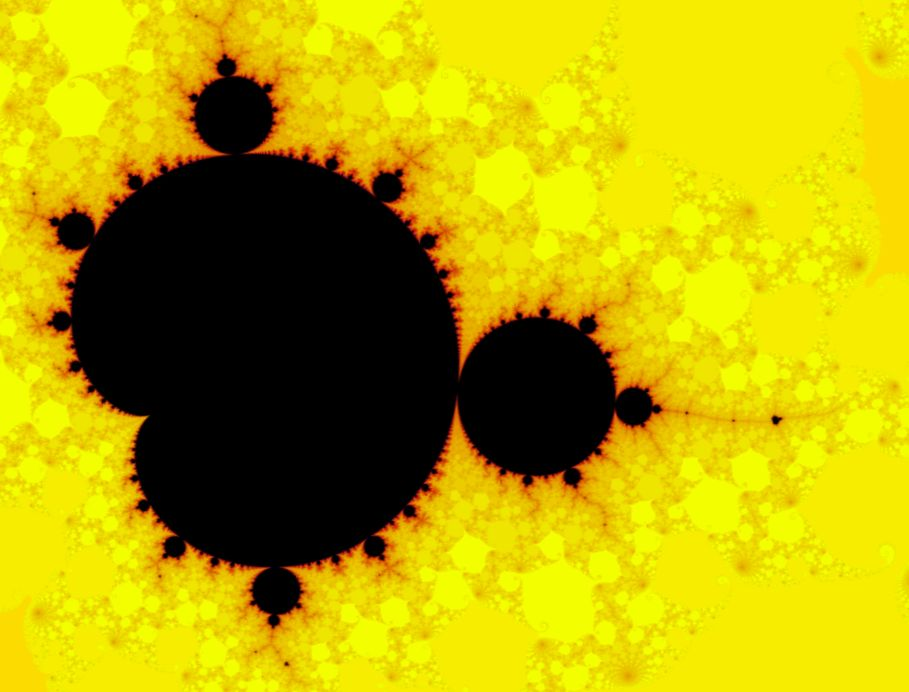
\includegraphics[width=.4\linewidth]{images/Mini_mandelbrot.jpg}}%
    \caption{Mandelbrot \cite{NormalMandelbrot} and a deformed "Mini-Mandelbrot" \cite{MiniMandelbrot}} %
    \label{fig:MandelbrotSet}%
\end{figure}%

\begin{figure}[!htbp]
    \centering
    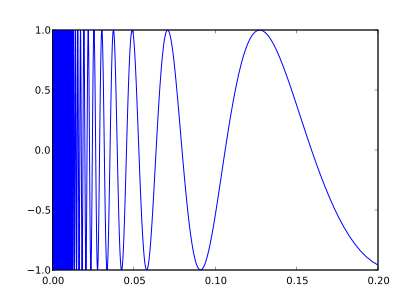
\includegraphics[width=.4\linewidth]{images/420px-Topologist_sine_curve.png}
    \caption{Topologist's Sine Curve \cite{TopSineCurve}}%\label{fig:boat1}
\end{figure}



\section{Mandelbrot Bound / Escape Radius}

Let $z_n = P_c^n(0)$,
\[ c \in M \iff \exists n \ni \abs{z_n} > 2\ \text{\cite{MandelbrotEscapeRadius}}\]

Given $\abs{z_n} > 2$, for $\abs{c} \leq 2$
\begin{align*}
    \abs{z_{n+1}} &\geq \abs{z_n}^2 - \abs{c} &&\text{Reverse Triangel Inequality} \\
    &\geq 2\abs{z_n} - 2 = \abs{z_n} + (\abs{z_n} - 2) \\
    &> \abs{z_n}
\end{align*}

For $\abs{c} > 2$, inductively $\abs{z_n} > \abs{c}$, so
\[ \abs{z_{n+1}} \geq \abs{z_n}^2 - \abs{c} > \abs{c}\abs{z_n} - \abs{c} > 2\abs{z_n} - \abs{c} > \abs{z_n} \] 


\section{Mandelbrot Fixed Points and Cycles}

\begin{itemize}
    \item "Main" Cardioid contains points whose sequence (orbit) approach attractive fixed point
    \begin{itemize}
        \item For fixed point $x^*$, $x_{n+1} = f(x_n) \approx f(x^*) + f'(x^*)(x_n - x^*)$
        \item $\abs{x_{n + 1} - x^*} = \abs{x_{n+1} - f(x^*)} \approx \abs{f'(x^*)}\abs{(x_n - x^*)}$
    \end{itemize}
    \item Other cardioids have cycles, periods labeled in Fig \ref{fig:MandelbrotCycles}
\end{itemize}

For $c$ with an attractive fixed point $z^*$ of $M$, we must have
\[ z^* = (z^*)^2 + c \]
and
\[ \abs{\frac{d}{dz}\Bigr|_{z^*}\left[z^2 + c\right]} < 1,\ \abs{z^*} < \frac{1}{2} \]
For $c$ on the boundary of those with fixed points, we have $\abs{z^*} = \frac{1}{2}$. Combining with the first condition, the solutions are the main cardioid curve.



\begin{figure}[!htbp]
    \centering
    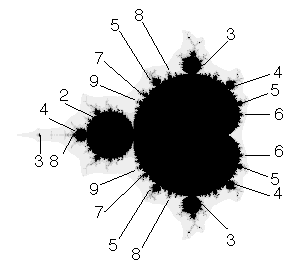
\includegraphics[width=.4\linewidth]{images/MandelMap1.png}
    \caption{Cardiods labeled with period \cite{MichaelFrame}} %\label{fig:boat1}
    \label{fig:MandelbrotCycles}
\end{figure}


\section{Visualizations}



\section{General Julia Sets}

Definitions
\begin{itemize}
    \item In general, iterating function $f(x) = p(x) / q(x)$ for complex polynomials $p, q$, no shared roots
    \begin{itemize}
        \item $f$ maps Riemann sphere onto itself
        \item $f$ is holomorphic
    \end{itemize}
    \item $f$ is invariant on open sets, Fatou Domains
    \item Fatou Set is union of Fatou Domains, it's dense!
    \item "True" Julia Set is the complement of the Fatou Set (boundary), also invariant
\end{itemize}

In the context of the Quadratic Julia Set described earlier...
\begin{itemize}
    \item "True" Julia Set is boundary of filled-in Julia Set
    \item Fatou Domains are...
        \begin{itemize}
            \item interior of filled-in Julia Set
            \item other side of Julia Set boundary, with unbounded orbit
        \end{itemize}
\end{itemize}


\section{Newton Fractals}

\begin{itemize}
    \item Newton method
    \begin{itemize}
        \item Iteratively approximate zeroes using tangent lines
        \item $x_{n+1} = x_n - p(x_n)/p'(x_n)$
        \item Works with complex functions
    \end{itemize}
    \item $f(x) = x - p(x)/p'(x)$ can be used as the iteration function for a Julia Set
    \item One Fatou Domain for each zero of $f$
    \item True Julia Set is the boundary where the method fails!
\end{itemize}


\begin{figure}[!htbp]
    %\setlength{\abovecaptionskip}{0pt}
    \centering
    \subfloat[$z^2 - 1$, two roots \cite{MichaelFrame}]{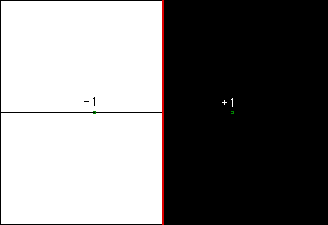
\includegraphics[width=.4\linewidth]{images/NewtonTwoRoots.png}}%
    \subfloat[$z^3 - 1$, three roots \cite{NewtonThreeRoots}]{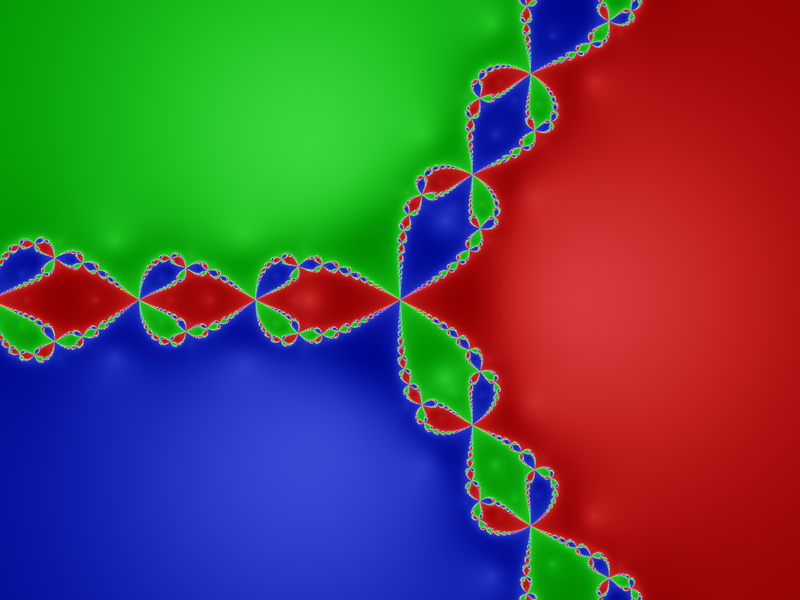
\includegraphics[width=.4\linewidth]{images/800px-Julia_set_for_three_roots.png}}%
    \caption{Newton's Method} %
    %\label{fig:M}%
\end{figure}%


\bibliographystyle{plain} % We choose the "plain" reference style
%\bibliographystyle{named}
\bibliography{refs} % Entries are in the "refs.bib" file

\end{document}
